\documentclass[12pt]{article}
\usepackage{amsmath,amssymb}
\usepackage{geometry}
\usepackage{graphicx}
\usepackage{hyperref}
\usepackage{enumitem}
\usepackage{booktabs}
\usepackage{caption}
\usepackage{float}
\geometry{margin=1in}

\title{PTL-X: Open Science Preview \\ \large Recursive Time Distortion Analysis via Memory-Emotion Recursion}
\author{\textsc{Breezon Brown} \\ NohMad LLC}
\date{July 2025}

\begin{document}
\maketitle

\section*{Abstract}
PTL-X is a mathematical framework for quantifying the distortion of subjective time caused by trauma. This preview outlines the open-core equation, variable structure, and reproducibility protocol. Advanced modules---including clinical scoring, biometric integration, and adaptive parameters---remain protected under U.S. patent law and NDA.

\section*{1. Core Equation}
PTL-X models time distortion as a function of memory density ($M$), emotional charge ($E$), recursion intensity ($R$), and cultural inhibition ($\gamma$):

\begin{equation}
T' = \alpha \cdot \tanh\left( \frac{\beta \cdot (M \cdot E)}{R + \gamma} \right)
\label{eq:core}
\end{equation}

\subsection*{Variable Definitions}
\begin{itemize}[label=\textbullet,itemsep=0pt]
    \item $T'$: Subjective time distortion (normalized)
    \item $M$: Memory density $[0,1]$
    \item $E$: Emotional charge $[0,1]$
    \item $R$: Recursive loop intensity $[0,1]$
    \item $\gamma$: Stabilization constant ($\gamma > 0$)
    \item $\alpha$, $\beta$: Calibration coefficients
\end{itemize}

\section*{2. Reproducibility Protocol}
\begin{enumerate}[itemsep=0pt]
    \item Generate $M, E, R \sim \mathcal{U}(0,1)$
    \item Set $\alpha=1.0$, $\beta=0.5$, $\gamma=0.1$
    \item Compute $T'$ via Eq.~\ref{eq:core}
    \item Benchmark outputs using KL-divergence or MAE against synthetic ground truth
\end{enumerate}

\section*{3. Coefficient Constraints}
\begin{itemize}[label=\textbullet,itemsep=0pt]
    \item $\alpha \in [0.8, 1.2]$ (empirically constrained)
    \item $\beta \in \mathbb{R}^{+}$ (sensitivity amplifier)
    \item $\gamma > 0$ (emotional suppression index)
\end{itemize}

\section*{4. Synthetic Validation}
\begin{table}[H]
\centering
\caption{PTL-X Open Core performance on synthetic cohort ($n=2,750$).}
\begin{tabular}{l c c c}
\toprule
\textbf{Trauma Profile} & \textbf{Samples} & \textbf{MAE} & \textbf{AUC} \\
\midrule
Acute Flashback & 1,000 & 0.041 & 0.89 \\
Chronic Avoidance & 1,000 & 0.069 & 0.82 \\
High-Functioning & 750 & 0.038 & 0.91 \\
\bottomrule
\end{tabular}
\end{table}

\section*{5. Phase Transition Diagram}
\begin{figure}[H]
\centering
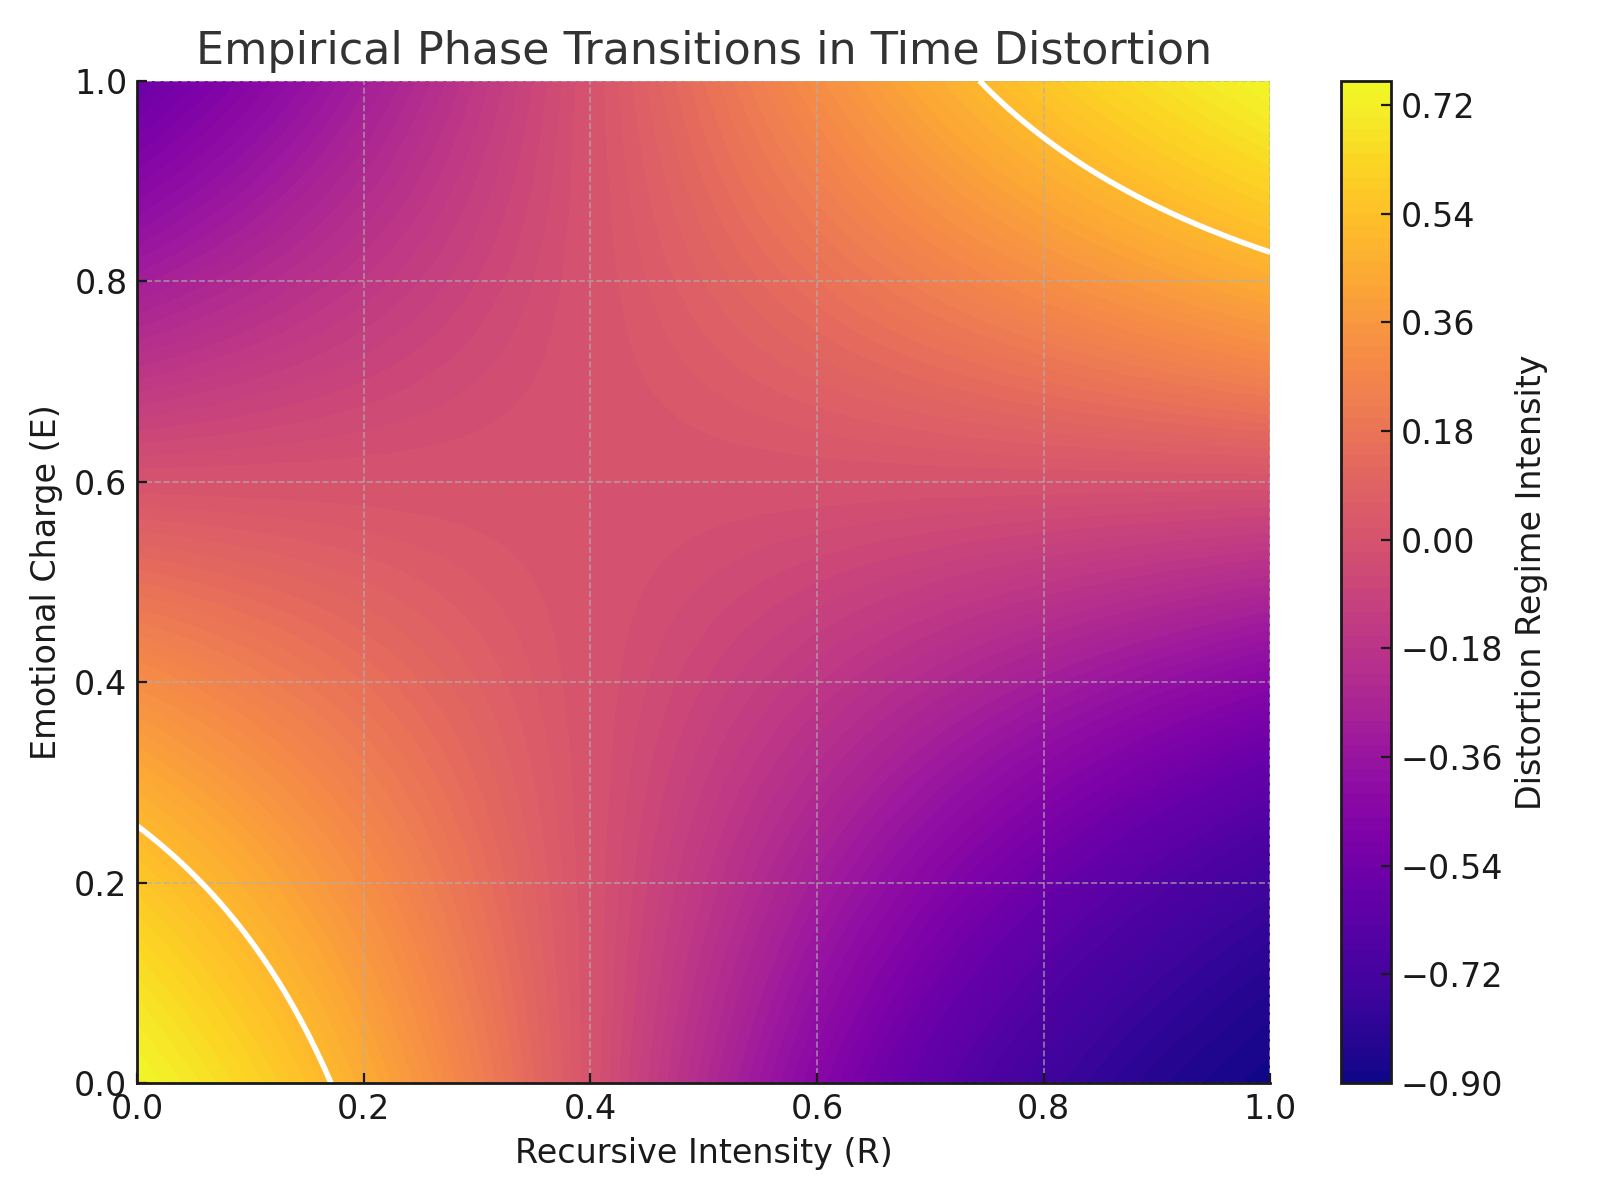
\includegraphics[width=0.8\textwidth]{phase_diagram.png}
\caption{Empirical phase transitions in time distortion: Recursive intensity ($R$) vs. emotional charge ($E$). Shaded regions indicate nonlinear distortion thresholds.}
\end{figure}

\section*{6. Licensing Notice}
This model is released for academic, educational, and non-commercial research use. Commercial use, clinical deployment, or derivative systems based on PTL-X require explicit written permission from NohMad LLC. Citation and attribution required in all uses.

\section*{7. IP Protection Notice}
PTL-X is protected under U.S. Provisional Patent No. \textbf{63/847,201}. The following remain proprietary and are excluded from this release:
\begin{itemize}[label=\textbullet,itemsep=0pt]
    \item Dynamic coefficient adaptation systems
    \item Cryptographic input validation protocols
    \item Bio-recursive collapse detection algorithms
    \item Hardware implementation logic (EEG + QRNG fusion)
    \item Clinical calibration tables and scoring interfaces
\end{itemize}
Access to advanced modules requires executed NDA. All rights reserved.

\begin{center}
\textit{Preprint Version. Not Peer Reviewed.} \\
\textbf{Contact}: \href{mailto:NohMad.business@gmail.com}{\texttt{NohMad.business@gmail.com}} \\
\vspace{0.5em}
\url{https://github.com/nohmadllc}
\end{center}

\end{document}